La struttura alla base del mio tirocinio è facile da comprendere, ma allo stesso tempo non lo è stata la realizzazione di tutte le operazioni che si trovano dietro ad esso, in particolare il calcolo dello zoom ideale per rappresentare una determinata area geografica e il sistema alla base del movimento e caricamento delle tile aggiornate in base alle direzioni di spostamento. Analizzando la struttura del progetto, troviamo una pagina HTML contente una form con i dati di partenza per ottenere la mappa dell'area prescelta, un server che elabori le cordinate dei punti inseriti e ne ricavi lo zoom corretto e infine si occupi dello streaming dell'immagine corretta e infine l'interfaccia 3D, sviluppata utilizzando la libreria \textit{Three.js} con cui l'utente può interagire per ottenere le mappe in seguito allo spostamento in direzione nord, sud, est e ovest.

\section{Modellazione delle informazioni}
La prima sfida affrontata nel corso dello sviluppo del seguente progetto è stata sicuramente il modo in cui un utente volesse interfacciarsi con il sistema. Pensando a come, spesso, vengono consultate le mappe nei vari sistemi online, risulta macchinoso trovare, a partire da un centro ipotetico, il modo di visualizzare una determinata area. Proprio per questo motivo, si è preferito affrontare la problema dando la possibilià all'utente di inserire le coordinate dei vertici della zona d'interesse. Risulta a questo punto immediato il calcolo del centro. Infatti una volta inseriti i due punti il centro avrà come cordinate il punto medio delle due cordinate di partenza. Considerando dunque due punti a e b di cordinate $(lat_{a}, long_{a})$ e $(lat_{b}, long_{b})$ il centro corrispondente sarà:
\begin{center}

	\LARGE$(\frac{lat_{a}+lat_{b}}{2} , \frac{long_{a}+long_{b}}{2})$\par

\end{center}
Il passo in questo è stato abbastanza semplice, perchè essendo il centro di un sistema di riferimento bidimensionale in punto medio tra due punti è la media delle cordinate dei due punti. Affrontando però la questione dello zoom e dello spostamento, la soluzione non è stata altrettanto diretta e semplice, tanto che le questioni saranno affrontate in due paragrafi distinti.

\subsection{Il calcolo dello zoom adatto}
Il calcolo dello zoom è stato il primo problema affrontato nel corso dell'implementazione e della progettazione del progetto. Lo zoom nelle mappe di Google è un valore discreto che varia da 0 a 21 e per comprenderne il funzionamento è stato necessario capire cosa venisse rappresentato ad ogni livello. Nella proiezione adottata da Google al livello 0 l'intero globo viene raffigurato in un'immagine di 256x256 pixels di larghezze e altezza. Questo ha rappresentato un valore di riferimento per lo studio della funzione che calcoli lo zoom di partenza. Andando, infatti, ad analizzare sperimentalmente i successivi livelli di zoom ho visto che ponendo lo zoom a 1, 256 pixels erano diventati troppo pochi per rappresentare l'intero globo. A questo grado di zoom infatti sono necessari esattamente 512 pixels di larghezza e altezza per rappresentare l'intera immagine terrestre, esattamente il doppio. L'ipotesi, dunque, a questo punto formulata vuole che lo zoom non è altro che una progressione geometrica di ragione 2. L'ipotesi è stata successivamente verificata analizzando anche il terzo grado di zoom, nonostante non fosse possibile mostrare un'immagine di 1024 pixels per lato in quanto le API di Google limitano l'utilizzo delle mappe statiche a dimensioni di 640 pixel per lato. È, dunque, possibile riassumere lo zoom di Google con la seguente espressione: 
\begin{center}

	\large$256\times2^{zoom}$\par

\end{center}
Ad ogni livello, dunque, corrispondono un certo numero di pixel capaci di contenere la rappresentazione dell'intero globo, come è possibile vedere in tabella:

\begin{center}
\begin{tabular}{c @{\hspace{1em}} c}
Livello	& Pixels \\

0 & 256\\
1 & 512\\
2 & 1024\\
...	& ...\\
z & $256\time2^z$\\
... & ...\\
21 & 536.870.912\\

\end{tabular}
\end{center}

E' risultato a questo punto quasi immediato calcolare lo zoom necessario a rappresentare una determinata area geografica. Infatti, in 256 pixel sono contenuti tutti i 360 gradi della circonferenza terrestre, considerando che la nostra immagine sarà di 640 pixels la proporzione è già costruita:
\begin{center}

	\LARGE$\frac{640}{\Delta} = \frac{256}{360} $\par

\end{center}
Il $\Delta$ della nostra funzione sarà in questo caso la variazione di \textbf{longitudine} tra i due punti richiesti dall'utente. Una variante della stessa proporzione, andrà utilizzata per la latitudine, dove i gradi da rappresentare non sono 360, bensì 180, o meglio per rispettare la proiezione utilizzata da Google 170,1022, perchè i poli in questo tipo di rappresentazione vengono considerati come due punti approssimati all'infinito non saremo quindi in grado di vedere interamente tutti i 180 gradi di latitudine che vanno dal polo nord al polo sud, besì ne verranno raffigurati 85,0511 rispettivamente a nord e a sud dell'equatore.

A questo punto, una volta ottenuto il risultato del rapporto, è opportuno calcolare lo zoom, che come abbiamo visto può essere rappresentato come una potenza in base due. Dunque per passare dalla nostra proporzione al livello di zoom richiesto occorrerà eseguire il logaritmo in base due del risultato della proporzione:
\begin{center}

	\Large$log_{2}(\frac{640}{\Delta}\times\frac{360}{256}) $\par

\end{center}

Una volta ottenuto lo zoom necessario, a questo punto sarà sufficiente concatenare i valori del centro e dello zoom all'url di richiesta della mappa, fornito dalle API di Google\footnote{Vedi Capitolo 4, Paragrafo 2.3} per poter caricare la mappa richiesta.

\subsection{Calcolo dei centri successivi per lo spostamento}
Se per lo zoom, i ragionamenti e i calcoli sono stati immediati, o quanto meno molto lineari, la stessa cosa non si può dire del calcolo dei nuovi centri per aggiornare la mia mappa nello spostamento lungo la longitudine e, soprattutto, la latitudine.

Perchè dover calcolare un nuovo centro? All'apparenza può risultare abbastanza inutile o eccessivo doversi calcolare un nuovo centro ad ogni spostamento. Essendo centro e zoom i due attributi necessari per caricare una mappa, questa rappresenterà solamente un certo spazio angolare della terra in relazione anche alla dimensione dell'immagine che viene richiesta, sia per quanto riguarda la latitudine che per quanto riguarda la longitudine. Sarà, dunque, necessario una volta raggiunto un certo margine della mappa, caricare la mappa successiva e di conseguenza occorrerà ricavarsi il centro per richiederla. Il problema principale, però è legato alla proiezione che Google ha deciso di utilizzare per rappresentare la terra in piano. Come si sa, la terra non è piana ma una sfera leggermente schiacciata ai due poli. Proprio per questo motivo, non è possibile direttamente rappresentare la terra su di una immagine piana, senza aver fatto le dovute proiezioni. Diversi sono stati i teorici che hanno elaborato delle proiezioni cartografiche del pianeta, ma in particolare il nostro studio ha riguardato la \textbf{la proiezione cilindrica centrografica modificata di Mercatore}, creata dal matematico e astronomo Gerhard Kremer e utilizzata da Google nella variante della \textit{Web Mercator Projection}.

All'inizio, inconsapevolmente si erano trattate latitudine e longitudine in maniera indistinta, è stata dunque elaborata una semplice proporzione tra gradi e pixel, derivata da quella per il calcolo dello zoom, al fine di trovare il centro della mappa successiva, sia essa a nord, sud, est oppure ovest. Per il movimento longitudinale, dunque verso oriente e occidente, non sono emersi problemi. Riprendendo la proporzione precedente sappiamo che se a 360 gradi corrispondono a 256 pixels moltiplicati per la potenza in base 2 dello zoom, allora in 640 pixel ci saranno una certa quantità di gradi. Se sommiamo questa quantità alla longitudine del nostro centro, ne ricaveremo quella del centro successivo a oriente.
Ricostruendo la formula si ha che:
\begin{center}

	\large$ (\frac{640\times360}{256\times2^{zoom}}) + longitudine_{c} $\par

\end{center}
dove $longitudine_{c}$ è la longitudine del centro da cui ci stiamo movendo. 

In egual misura, se ci stiamo movendo verso occidente, sottraendo la stessa quantità alla longitudine del centro di partenza otterremo il nostro centro ad occidente:
\begin{center}

	\large$  longitudine_{c} - (\frac{640\times360}{256\times2^{zoom}}) $\par

\end{center}

Inizialmente, l'idea è stata applicata anche alla latitudine, muovendosi verso nord e verso sud. Ovviamente in questo caso la proporzione era stata modificata considerando i 170,1022 gradi complessivi dei paralleli terrestri. La funzione verrebbe così riprodotta:
\begin{center}

	\large$  latitudine_{c} \pm (\frac{640\times360}{256\times2^{zoom}}) $\par

\end{center}

I risultati inizialmente ottenuti non sono stati però quelli sperati. Il centro calcolato risultava sempre spostato, creando duplicazioni di alcune zone geografiche o a volte, addirittura, il completo taglio di altre. Dopo diversi fallimentari tentativi di approssimare il più possibile il calcolo, utilizzando, o teorizzando in alcuni casi, anche delle funzioni che in base alla latitudine approssimassero il punto in cui attaccare le mappe presenti sulla canvas. La risposta è stata trovata, alla fine, studiando la stessa proiezione di Mercatore.

Per la proiezione, un grado di latitudine all'equatore non vale quanto un grado di latitudine ai poli, questo è dovuto principalmente al diverso grado di distorsione presente in distinte aree geografiche della terra. Una rappresentazione di quanto appena detto può essere visto nell'immagine \ref{fig:mercatorproj}
\begin{figure}[H]
	\centering
	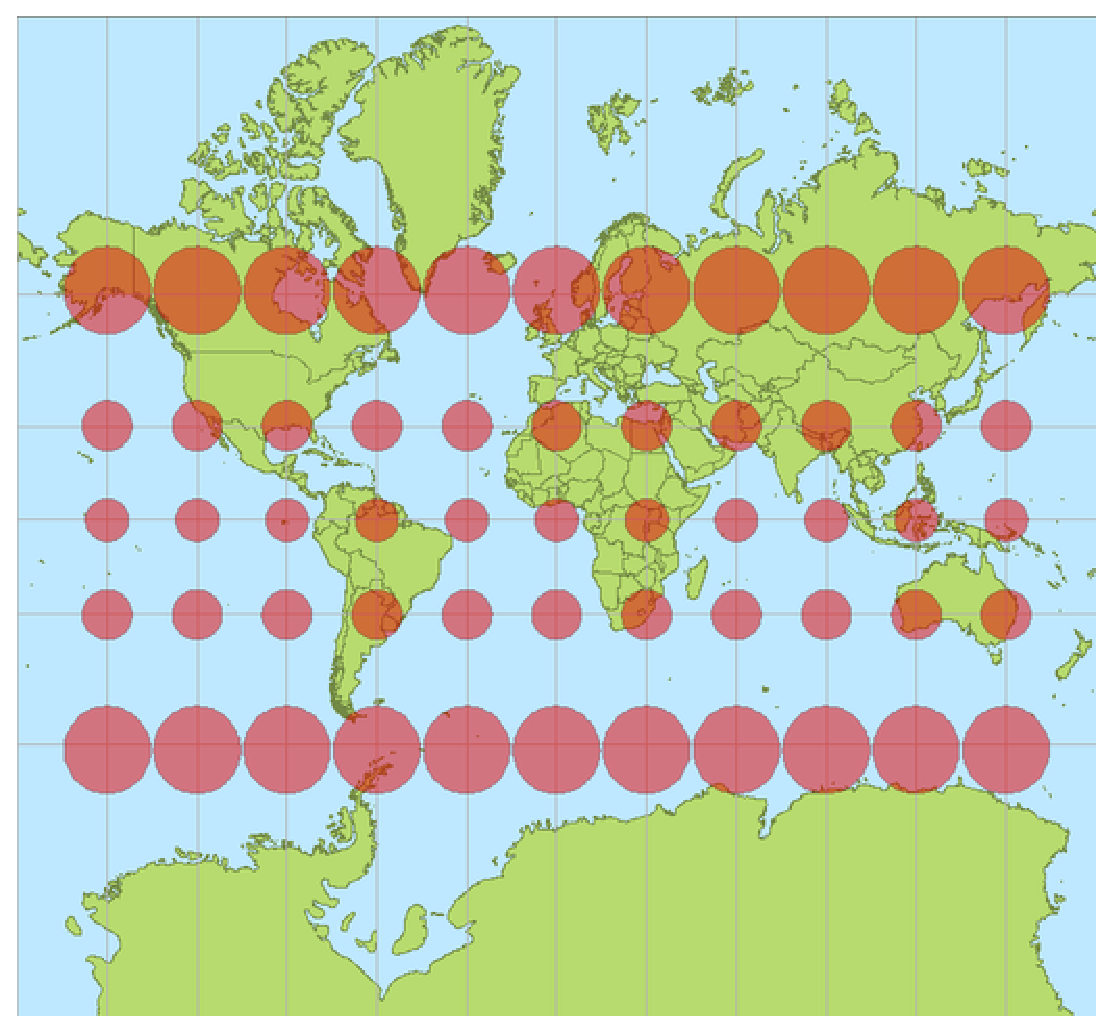
\includegraphics[scale=0.5]{figure/mercatorproj.eps}
	\caption{Rappresentazione della distorsione delle aree geografiche}\label{fig:mercatorproj}
\end{figure}

Seguendo questa proiezione, per effettuare i calcoli è stato necessario effettuare diverse conversioni. In primo luogo quella tra gradi decimali e radianti seguendo una semplice proporzione:
\begin{center}

	\Large$ \frac{deg}{180} = \frac{rad}{\pi} $\par

\end{center}

A questo punto è stato necessario applicare le conversioni forniteci dallo stesso Mercatore, per comprendere quale fosse il centro successivo a nord e a sud. 

Per prima cosa, occorre passare dal sistema di riferimento geoassiale al sistema in pixel utilizzando la seguente formula di conversione:
\begin{center}

	\large$ \frac{1}{2}ln(\frac{1+\sin(lat)}{1-\sin(lat)}) $

\end{center}
Una volta ottenuto questo valore, per ottenere la conversione sarà necessario aggiungerci la metà della dimensione del globo terrestre, in pixel, secondo quella che è la dimensione di riferimento della proiezione, ovvero 256 pixels. La formula, quindi, riassunta è la seguente:
\begin{center}

	\large$ 128 + \frac{1}{2}ln(\frac{1+\sin(lat)}{1-\sin(lat)}) $

\end{center}